\section{Antwort}

S. Abbildung~\ref{fig:aufgabe2}.\\

\begin{figure}
    \centering
    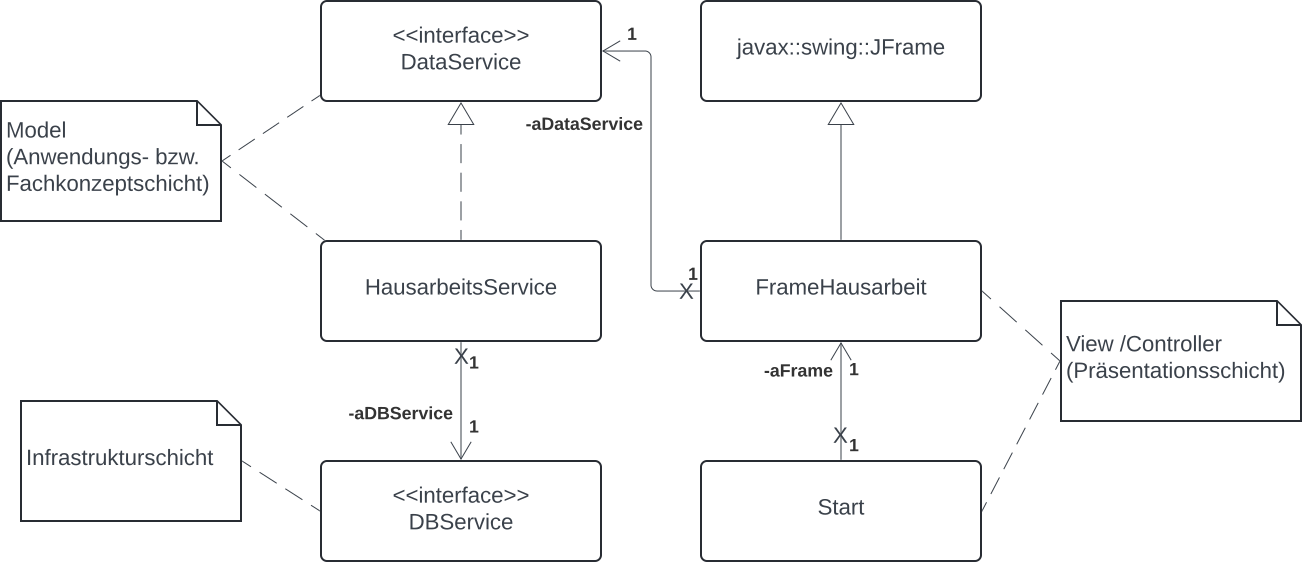
\includegraphics[scale=0.5]{chapters/aufgabe 2/img/aufgabe2}
    \caption{UML für den in Aufgabe 2 verkürzt dargestellten Quellcode. (Quelle: eigene)}
    \label{fig:aufgabe2}
\end{figure}

\subsection{Anmerkungen}
Explizite Angaben zu Multiplizität und Navigierbarkeit können in einem \textbf{Feinentwurf} ergänzt werden (vgl.~\cite[415]{Bal05}). Auf den Feinentwurf folgt die Implementierung.\\

\subsubsection*{Multiplizitäten}
Da der Quellcode (als mögliches Ergebnis eines Feinentwurf) in der Aufgabe verkürzt dargestellt ist, kann keine genaue Aussage zur Multiplizität getroffen werden - es geht aus dem Quelltext also nicht \textit{eindeutig} hervor, ob es sich bei den Assoziationen um \textbf{Kann}- oder \textbf{Muss}-Beziehungen handelt: Bei einer einseitigen \textbf{Muss}-Beziehung von Objekt \code{A} zu Objekt \code{B} muss bspw. die Beziehung zu Objekt \code{B} aufgebaut werden, sobald Objekt \code{A} erzeugt wird (vgl.~\cite[43]{Bal05}) - hierzu fehlt aber zumindest der Konstruktor, der dazu mehr Informationen liefern könnte.\\

\noindent
Würden wir die Multiplizität in dem resultierenden UML-Diagramm nicht angeben, wäre die Multiplizität implizit \code{[1]}\footnote{
    \textit{Fowler} empfiehlt diesbzgl. in \cite[39]{Fow03b} ``The default implicity of an attribute is [1]. Although this is true in the meta-model,you can't assume that an attribute in a diagram that's missing a multiplicity has a value of [1], as the diagram may be suppressing the multiplicity information. As a result, I prefer to explicitly state a [1] multiplicity if it's important.``
    }:
\blockquote[{\cite[19]{OMG17}}]{
If no multiplicity is shown on an association end, it implies a multiplicity of exactly 1. (\cite[19]{OMG17})
}.

\noindent
Bei der Lösung gehen wir also von \textbf{Muss-Beziehungen} aus: Die Anwendung kann nicht ohne den View (\code{FrameHausarbeit}) existieren, der View benötigt das Model (\code{DataService}), das Model den Zugriff auf die Datenhaltung (\code{DBService}).\\
Im besten Fall ist die Verteilung der Services über \textbf{Dependency Injection} geregelt - in unserem Fall gehen wir von Konstruktor-basierter DI aus\footnote{
\url{https://martinfowler.com/articles/injection.html#ConstructorInjectionWithPicocontainer}, abgerufen 17.05.2024
}.

\subsubsection*{Navigierbarkeit}
Die meisten Assoziationsrichtungen lassen sich aus dem Quelltext entnehmen, so dass wir in allen Fällen \textit{unidirektionale} Assoziationen erstellen können: So greifen bspw. Objekte der Klasse \code{Start} über eine Referenz auf \code{FrameHausarbeit} zu.\\
Wollen wir die \textbf{Navigierbarkeit} in umgekehrter Richtung \textit{explizit} ausschließen, müssen wir noch die \textit{nonNavigableNotation}\footnote{
    zur Verwendung der \textit{navigabilityNotation}- und \textit{nonNavigabilityNotation}-Notationselemente zur expliziten Darstellung der Navigierbarkeit s.~\cite[203]{OMG17}
}-Notation verwenden - ansonsten ist die andere Richtung \textit{undefiniert} (vgl.~\cite[285]{Bal05})\footnote{
    Bzgl. der in der UML-Spezifikation vereinbarten Konventionen: ``Arrow notation is used to denote association end navigability. By definition, all class-owned association ends are navigable. By convention, all association-owned ends in the metamodel are not navigable.`` (\cite[18]{OMG17}) sowie ``An association with neither end marked by navigability arrows means that the association is navigable in both directions.`` (\cite[19]{OMG17})
}.\\
Dies tun wir aber auch für alle Assoziationen und begründen dies an dieser Stelle mit der geg. Semantik der vorhandenen Klassen und Schnittstellen:

\begin{itemize}
    \item \code{Start} und \code{FrameHausarbeit} verorten wir in einer Mehr-Schichten-Architektur (\cite[31 ff.]{BMRS96}) in die \textbf{Präsentations}-Schicht, insb. hier \code{FrameHausarbeit} als Teil des \textbf{View}s.
    \item[] Da \code{Start} Verantwortlichkeiten eines \textbf{Controller}s übernimmt (Anzeige Haupt-Ansicht etc.), wäre ein Zugriff in diese Richtung von \code{FrameHausarbeit} möglich (vgl.~\cite[128]{BMRS96}), wir entscheiden uns, die Assoziationsrichtung \textit{undefiniert} zu lassen
    \item \code{HausarbeitsService} realisiert \code{DataService}, weshalb wir davon ausgehen, dass diese Klasse Teil des \textbf{Models} ist.
    Als Komponente einer Fachkonzeptschicht (\cite[409 f.]{Bal05}) sowie als \textbf{Model} im \textbf{MVC}-Muster ist ein Zugriff auf die \textbf{View}-Componente (\code{FrameHausarbeit}) ausgeschlossen, was wir im Klassendiagramm durch die Notation explizit zum Ausdruck bringen
    \item \code{DBService} ermöglicht Zugriffe auf die Datenhaltung und ist deshalb Teil der \textbf{Infrastruktur}-Schicht.
    Auch hier sind die Zugriffe auf überliegende Schichten klar geregelt, weshalb auch hier eine Navigierbarkeit in Richtung \code{HausarbeitsService} explizit ausgeschlossen wird\footnote{
    \textit{Buschmann et al.} beschreiben mehrere Szenarien, wie der Zugriff auf die Schichten geschieht (\cite[36]{BMRS96}). Neben dem Top-Down-Approach ist   auch die umgekehrte Richtung über Benachrichtigungen möglich, wobei die Implementierung der einzelnen Schichten gemein haben, dass die unterliegenden Schichten nichts von der darüberliegenden Schichten wissen, sondern nur umgekehrkt: Die Kopplung erfolgt in eine Richtung  (\cite[41]{BMRS96}). Bottom-Up-Szenarien können dann über \textit{Callbacks} realisiert werden, also bspw. unter Verwendung des \textbf{Observer}-Patterns.
    Diese Art der direkten/indirekten Kommunikation in einer \textit{Layered-Architecture} greift auch \textit{Evans} in ~\cite[68]{Eva03} auf.
     }
\end{itemize}
